\subsection{積分定理}
	本稿では,複素数$z$と$w$に対して
	\begin{align}
		[0,1] \ni t \longmapsto z + t \cdot (w - z)
	\end{align}
	なる写像を
	\begin{align}
		\seg{z}{w}
	\end{align}
	と表す.つまり
	\begin{align}
		\seg{z}{w} \defeq \Set{(t,\zeta)}{t \in [0,1] \wedge \zeta = z + t \cdot (w - z)}
	\end{align}
	と定めている.$\seg{z}{w}$とは$z$と$w$を結ぶ線分を描き,また$f$をその線分上の連続写像とすれば
	\begin{align}
		\int_{\seg{z}{w}} f = (w-z) \cdot \int_{[0,1]} f(z + t \cdot (w - z))\ dt
	\end{align}
	が成り立つ.また$t$を$[0,1]$の要素とすれば
	\begin{align}
		\seg{w}{z}(t) = \seg{z}{w}(1 - t)
	\end{align}
	が成り立つので,$\seg{w}{z}$は$\seg{z}{w}$の逆路である.ゆえに
	\begin{align}
		\int_{\seg{w}{z}} f = - \int_{\seg{z}{w}} f
	\end{align}
	が成立する.
	
	いま$a$と$b$と$c$を複素数とすると,
	\begin{align}
		\Delta \defeq \Set{z}{\exists t,s \in [0,1]\, 
		\left(\, z = (1-t) \cdot a 
		+ t \cdot (1-s) \cdot b 
		+ t \cdot s \cdot c\, \right)}
	\end{align}
	により定める集合$\Delta$は,イメージとしては$a,b,c$によって囲まれる三角形
	
	\begin{center}
	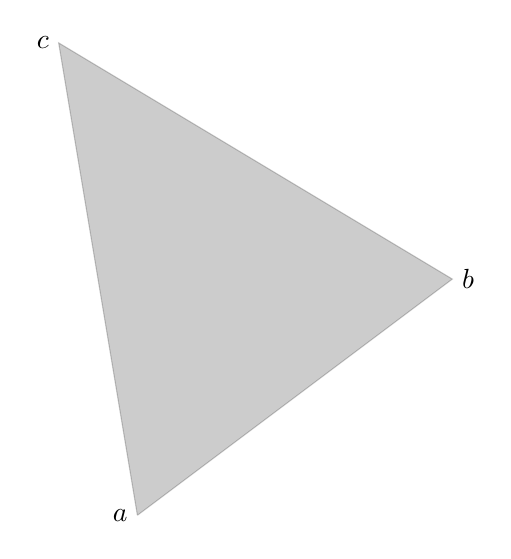
\begin{tikzpicture}
		\filldraw[opacity=0.2] (0,0)--(4,3)--(-1,6)--(0,0);
		\node[anchor=east] at (0,0) {$a$};
		\node[anchor=west] at (4,3) {$b$};
		\node[anchor=east] at (-1,6) {$c$};
	\end{tikzpicture}
	\end{center}
	
	を表す.この$\Delta$は$\C$のコンパクト部分集合である.実際,
	\begin{align}
		(t,s) \longmapsto (1-t) \cdot a + t \cdot (1-s) \cdot b + t \cdot s \cdot c
	\end{align}
	は$\R^2$から$\C$への連続写像であって,$\Delta$とはこの写像によって
	\begin{align}
		[0,1] \times [0,1]
	\end{align}
	なる$\R^2$のコンパクト部分集合を写した像である.
	
	三角領域の外郭に沿った正則関数の線積分は$0$になる.
	
	\begin{screen}
		\begin{thm}[Goursat]\label{Cauchy_Goursat_theorem}
			$a$と$b$と$c$を複素数とし,
			\begin{align}
				\Delta \defeq \Set{z}{\exists t,s \in [0,1]\, 
				\left(\, z = (1-t) \cdot a 
				+ t \cdot (1-s) \cdot b 
				+ t \cdot s \cdot c\, \right)}
			\end{align}
			と定める.また$\Omega$を$\C$の開集合とし,
			$f$を$\Omega$上の$\C$値連続写像とし,$p$を$\Omega$の要素とする.
			このとき,
			\begin{align}
				\Delta \subset \Omega
			\end{align}
			かつ,$p$を除く$\Omega$の各要素で$f$が微分可能であれば
			\begin{align}
				\int_{\seg{a}{b}} f + \int_{\seg{b}{c}} f + \int_{\seg{c}{a}} f = 0.
			\end{align}
		\end{thm}
	\end{screen}
	
	\begin{screen}
		\begin{thm}[凸開集合に含まれる任意の三角形の周上の積分が$0$である連続写像は正則関数の導関数]
		\label{thm:a_holomorphic_function_is_derivative_of_some_holomorphic_function_on_convex_open}
			$\Omega$を$\C$の凸開集合とし,$f$を$\Omega$上の$\C$値連続写像とする.
			このとき,$\Omega$の任意の三要素$a$と$b$と$c$に対して
			\begin{align}
				\int_{\seg{a}{b}} f + \int_{\seg{b}{c}} f + \int_{\seg{c}{a}} f = 0
			\end{align}
			が満たされているならば,$p$を$\Omega$の要素として$F$を
			\begin{align}
				\Omega \ni z \longmapsto \int_{\seg{p}{z}} f
			\end{align}
			なる関係により定める写像とすれば
			\begin{align}
				F' = f
			\end{align}
			が成立する.
		\end{thm}
	\end{screen}
	
	\begin{sketch}
		$\Omega$の任意の三要素$a$と$b$と$c$に対して
		\begin{align}
			\int_{\seg{a}{b}} f + \int_{\seg{b}{c}} f + \int_{\seg{c}{a}} f = 0
		\end{align}
		が満たされているとする.また$p$を$\Omega$の要素として,
		\begin{align}
			\Omega \ni z \longmapsto \int_{\seg{p}{z}} f
		\end{align}
		なる写像を$F$とする.$z$と$w$を$\Omega$の要素とすれば
		\begin{align}
			\int_{\seg{z}{w}} f = -\int_{\seg{w}{p}} f - \int_{\seg{z}{p}} f
		\end{align}
		が成り立つが,
		\begin{align}
			\int_{\seg{w}{p}} f = -\int_{\seg{p}{w}} f = -F(w)
		\end{align}
		より
		\begin{align}
			\int_{\seg{z}{w}} f = F(w) - F(z)
		\end{align}
		が得られる.よって,$h$を
		\begin{align}
			z + h \in \Omega
		\end{align}
		である範囲の任意の複素数とすれば
		\begin{align}
			F(z+h) - F(z) - h \cdot f(z)
			&= \int_{\seg{z}{z+h}} f - h \cdot f(z) \\
			&= h \cdot \int_{[0,1]} f(z + t \cdot h) - f(z)\ dt
		\end{align}
		が成立する.ところで$f$は$z$で連続であるから,いま$\epsilon$を任意に与えられた正の実数とすれば
		\begin{align}
			|h| < \delta \Longrightarrow |f(z+h) - f(z)| < \epsilon
		\end{align}
		を満たす正の実数$\delta$が取れる.そして$h$を
		\begin{align}
			|h| < \delta
		\end{align}
		を満たす任意の複素数とすれば
		\begin{align}
			|F(z+h) - F(z) - h \cdot f(z)|
			\leq |h| \cdot \int_{[0,1]} |f(z + t \cdot h) - f(z)|\ dt
			< |h| \cdot \epsilon
		\end{align}
		が成り立つ.ゆえに$F$は$z$で微分可能であり,その微分係数は
		\begin{align}
			f(z)
		\end{align}
		である.
		\QED
	\end{sketch}
	
	\begin{screen}
		\begin{thm}[円周上の積分公式]
			$\Omega$を開集合とし,$f$を$\Omega$上の正則関数とし,$z$を$\Omega$の要素とし,
			\begin{align}
				R \defeq \inf{}{\Set{|z-w|}{w \in \C \wedge w \notin \Omega}}
			\end{align}
			とする.つまり$R$とは$z$と$\C \backslash \Omega$との距離である.このとき$r$を
			\begin{align}
				0 < r < R
			\end{align}
			を満たす任意の実数として,$\gamma$を
			\begin{align}
				[0,2 \cdot \pi] \ni \theta \longmapsto z + r \cdot e^{\isym \cdot \theta}
			\end{align}
			なる写像とすれば,
			\begin{align}
				f(z) = \frac{1}{2 \cdot \pi \cdot \isym} \cdot \int_{\gamma} \frac{f(w)}{w - z}\ dw
			\end{align}
			が成立する.
		\end{thm}
	\end{screen}
	
	\begin{sketch}
		$\Omega$上の写像$g$を
		\begin{align}
			\Omega \ni w \longmapsto
			\begin{cases}
				\displaystyle{\frac{f(w) - f(z)}{w - z}} & \mbox{if } w \neq z \\
				f'(z) & \mbox{if } w = z
			\end{cases}
		\end{align}
		なる関係により定めると,$g$は$\Omega$上で連続であって
		\begin{align}
			g \in \Holomorphic{\Omega \backslash \{z\}}
		\end{align}
		を満たすので,定理\ref{Cauchy_Goursat_theorem}と
		定理\ref{thm:a_holomorphic_function_is_derivative_of_some_holomorphic_function_on_convex_open}より
		$\disc{z}{R}$の各要素$w$で
		\begin{align}
			G'(w) = g(w)
		\end{align}
		を満たす$\disc{z}{R}$上の正則関数$G$が取れる.$r$を
		\begin{align}
			0 < r < R
		\end{align}
		なる実数とし,$\gamma$を
		\begin{align}
			[0,2 \cdot \pi] \ni \theta \longmapsto z + r \cdot e^{\isym \cdot \theta}
		\end{align}
		なる写像とすれば,微分積分学の基本定理より
		\begin{align}
			\int_{\gamma} g
			&= \int_{[0,2 \cdot \pi]} g(\gamma(\theta)) \cdot \gamma'(\theta)\ d\theta \\
			&= \int_{[0,2 \cdot \pi]} G'(\gamma(\theta)) \cdot \gamma'(\theta)\ d\theta \\
			&= G(\gamma(2 \cdot \pi)) - G(\gamma(0)) \\
			&= G(z + r) - G(z + r) \\
			&= 0
		\end{align}
		が成立する.ゆえに
		\begin{align}
			\int_{\gamma} \frac{f(w)}{w - z}\ dw 
			&= f(z) \cdot \int_{\gamma} \frac{1}{w - z}\ dw \\
			&= f(z) \cdot \int_{[0,2\cdot\pi]} \frac{r \cdot \isym \cdot e^{\isym \cdot \theta}}{r \cdot e^{\isym \cdot \theta}} d\theta \\
			&= (2 \cdot \pi \cdot \isym) \cdot f(z)
		\end{align}
		が成立する.
		\QED
	\end{sketch}
	
	Goursatの定理の逆が成立する.
	\begin{screen}
		\begin{thm}[Moreraの定理]
			
		\end{thm}
	\end{screen}
	
	\begin{screen}
		\begin{thm}[Cauchyの積分定理]
			$\Omega$を開集合とし,$f$を$\Omega$上の正則関数とし,$\gamma$を路とする.このとき,
			\begin{align}
				\ran{\gamma} \subset \Omega
			\end{align}
			かつ
			\begin{align}
				\forall z \in \C \backslash \Omega\, \left(\, \Ind_{\gamma}(z) = 0\, \right)
			\end{align}
			が満たされていれば,$\Omega \backslash \ran{\gamma}$の任意の要素$z$に対して
			\begin{align}
				f(z) \cdot \Ind_{\gamma}(z) = \frac{1}{2\cdot\pi\cdot\isym} \cdot \int_{\gamma} \frac{f(w)}{w - z}\ dw
			\end{align}
			が成立する.特に
			\begin{align}
				\int_\gamma f = 0
			\end{align}
			が成立する.
		\end{thm}
	\end{screen}
	
	\begin{sketch}[大雑把]
		$\Omega \times \Omega$上の写像$g$を
		\begin{align}
			\Omega \times \Omega \ni (z,w) \longmapsto
			\begin{cases}
				{\displaystyle \frac{f(w) - f(z)}{w-z}} & \mbox{if } z \neq w \\
				f'(z) & \mbox{if } z = w
			\end{cases}
		\end{align}
		により定めれば,$g$は連続である.
		\begin{align}
			\Omega \ni z \longmapsto \frac{1}{2\cdot\pi\cdot\isym} \cdot \int_{\gamma} \frac{f(w)-f(z)}{w-z}\ dw
		\end{align}
		なる写像を$h$とすれば$h$は連続である.$a,b,c$を$\Omega$の要素として,それらがなす三角集合が$\Omega$に含まれるとき,つまり
		\begin{align}
			\Set{z}{\exists t,s \in [0,1]\, 
			\left(\, z = (1-t) \cdot a 
			+ t \cdot (1-s) \cdot b 
			+ t \cdot s \cdot c\, \right)} \subset \Omega
		\end{align}
		なるとき,Fubiniの定理とGoursatの定理より
		\begin{align}
			&\int_{\seg{a}{b}} h + \int_{\seg{b}{c}} h + \int_{\seg{c}{a}} h \\
			&= \frac{1}{2 \cdot \pi \cdot \isym} \cdot \int_{\gamma} 
			\left(\int_{\seg{a}{b}} g_w + \int_{\seg{b}{c}} g_w + \int_{\seg{c}{a}} g_w\right)\ dw \\
			&= 0
		\end{align}
		が成立するので,Moreraの定理より
		\begin{align}
			h \in \Holomorphic{\Omega}
		\end{align}
		が従う.
		\begin{align}
			\Psi \defeq \Ind_{\gamma}^{-1} \ast \{0\}
		\end{align}
		により$\C$の開集合を定めて
		\begin{align}
			\C \ni z \longmapsto
			\begin{cases}
				{\displaystyle \frac{1}{2\cdot\pi\cdot\isym} \cdot \int_{\gamma} \frac{f(w)-f(z)}{w-z}\ dw} & \mbox{if } z \in \Omega \\
				{\displaystyle \frac{1}{2\cdot\pi\cdot\isym} \cdot \int_{\gamma} \frac{f(w)}{w-z}\ dw} & \mbox{if } z \in \Psi
			\end{cases}
		\end{align}
		なる写像を$\varphi$とすると,$\varphi$は整関数であって,
		\begin{align}
			\lim_{|z| \longrightarrow \infty} \varphi(z) = 0 
		\end{align}
		であるから
		\begin{align}
			\forall z \in \C\, (\, \varphi(z) = 0\, )
		\end{align}
		が成立する.ゆえに$\Omega \backslash \ran{\gamma}$の任意の要素$z$に対して
		\begin{align}
			\frac{1}{2\cdot\pi\cdot\isym} \cdot \int_{\gamma} \frac{f(w)-f(z)}{w-z}\ dw = 0
		\end{align}
		が成立するから,移項して
		\begin{align}
			\frac{1}{2\cdot\pi\cdot\isym} \cdot \int_{\gamma} \frac{f(w)}{w-z}\ dw
			= f(z) \cdot \Ind_{\gamma}(z)
		\end{align}
		を得る.$\Omega \backslash \ran{\gamma}$の要素$z$を取り
		\begin{align}
			\Omega \ni w \longmapsto f(w) \cdot (w - z)
		\end{align}
		なる写像を$F$と定めれば,
		\begin{align}
			F \in \Holomorphic{\Omega}
		\end{align}
		であるから
		\begin{align}
			\int_{\gamma} f = \int_{\gamma} \frac{F(w)}{w-z}\ dw = F(z) \cdot \Ind_{\gamma}(z) = 0
		\end{align}
		が成立する.
		\QED
	\end{sketch}